\section{Объясняющее двоичное дерево eXBTree}\label{sec:ch1/exbtree}

%%%%%%%%%%%%%%%%%%%%%%%%%%%%%%%%%%%%%%%%%%%%%%%%%%%%%%%%%%%%%%%%%%%%%%%%%%%%%%%%%%%%%%%%%%%%%%%%%%%%%%%%%%%%%%%
\subsection{Построение объясняющего дерева решений}

Как было сказано в разделе~\cref{subsec:ch1/neural_approximation}, многослойный персептрон с кусочно-линейной функцией активации разбивает входное пространство признаков на \(N\) непересекающихся ячеек \(\{K_1, K_2, \ldots, K_N\}\). В каждой такой ячейке значение выходного нейрона определяется фиксированной линейной комбинацией признаков.

Рассмотрим полносвязный персептрон с \(L\) скрытыми слоями по \(k\) нейронов в каждом. В качестве функции активации используется модуль: 
\[
\sigma(z) = |z|.
\]

Обозначим выходы нейронов первого скрытого слоя через \(A_i\), второго -- через \(B_i\), третьего -- через \(C_i\), и так далее (рисунок~\cref{fig:perceptron_architecture}). Для произвольного нейрона слоя \(A\) выполняется:
\[
A_i = \left| \sum_{j=1}^{d} a_{ij} x_j + a_{i0} \right|,
\]
где \( x \in [0, 1]^d \) -- входной вектор признаков. Аналогично, для следующего слоя:
\[
B_i = \left| \sum_{j=1}^{k} b_{ij} A_j + b_{i0} \right|,
\]
и так далее до выходного слоя:
\[
    c_n(x) = \sum_{j=1}^{k} c_{j} B_j + c_{0}.
\]

\begin{figure}[ht]
    \centerfloat{
        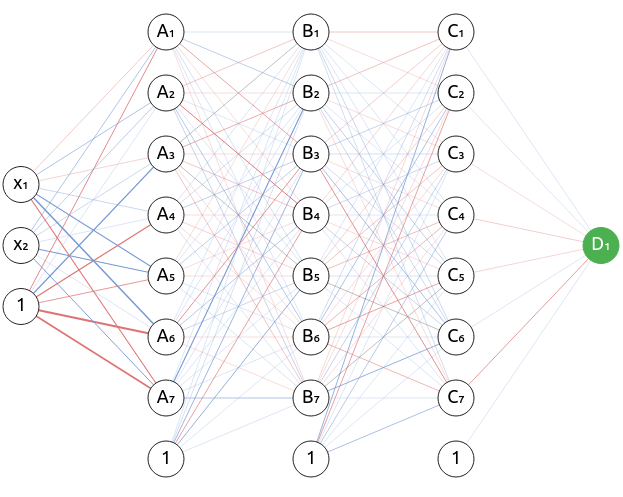
\includegraphics[width=\linewidth]{Dissertation/images/ch1/exbtree/perceptron.png}
    }
    \caption{Архитектура многослойного персептрона с \(d=2\), \(L=3\), \(k=7\)}
    \label{fig:perceptron_architecture}
\end{figure}

Каждый нейрон разбивает своё входное пространство на две области: одну, в которой входная сумма положительна (в этом случае модуль раскрывается со знаком «плюс»), и другую, где сумма отрицательна (в этом случае модуль раскрывается со знаком «минус»). Таким образом, на каждом шаге можно заменить модуль линейным выражением с соответствующим знаком.

Пошагово раскрывая модули в нейронах первого слоя, можно сформировать дерево, в котором каждый путь соответствует определённой комбинации знаков раскрытия модулей. В узлах дерева находятся неравенства, задаваемые условиями перехода: при переходе по левой ветви знак раскрытия модуля в текущем нейроне отрицателен, по правой -- положителен. После обработки всех нейронов слоя \(A\) все функции активации будут раскрыты, и входы к следующему слою \(B\) становятся кусочно-линейными выражениями, зависящими от исходных переменных \(x_j\), и процесс повторяется.

Таким образом, можно построить объясняющее двоичное дерево решений~\cite{song2015decision}, в дальнейшем называемое \textbf{eXBTree} (eXplanatory Binary Tree), в котором каждая вершина соответствует разбиению пространства по линейному неравенству одного нейрона, а каждая листовая вершина -- конечной линейной функции выходного слоя, полученной на конкретной ячейке пространства. Последовательность знаков, с которыми раскрывались активационные функции нейронов по пути от входа к выходному нейрону кодирует произвольную ветку в построенном дереве (рисунок~\cref{fig:exbtree_example}).

\nomenclature{eXBTree}{двоичное дерево решений, построенное на основе многослойного персептрона}

\begin{figure}[ht]
    \centerfloat{
        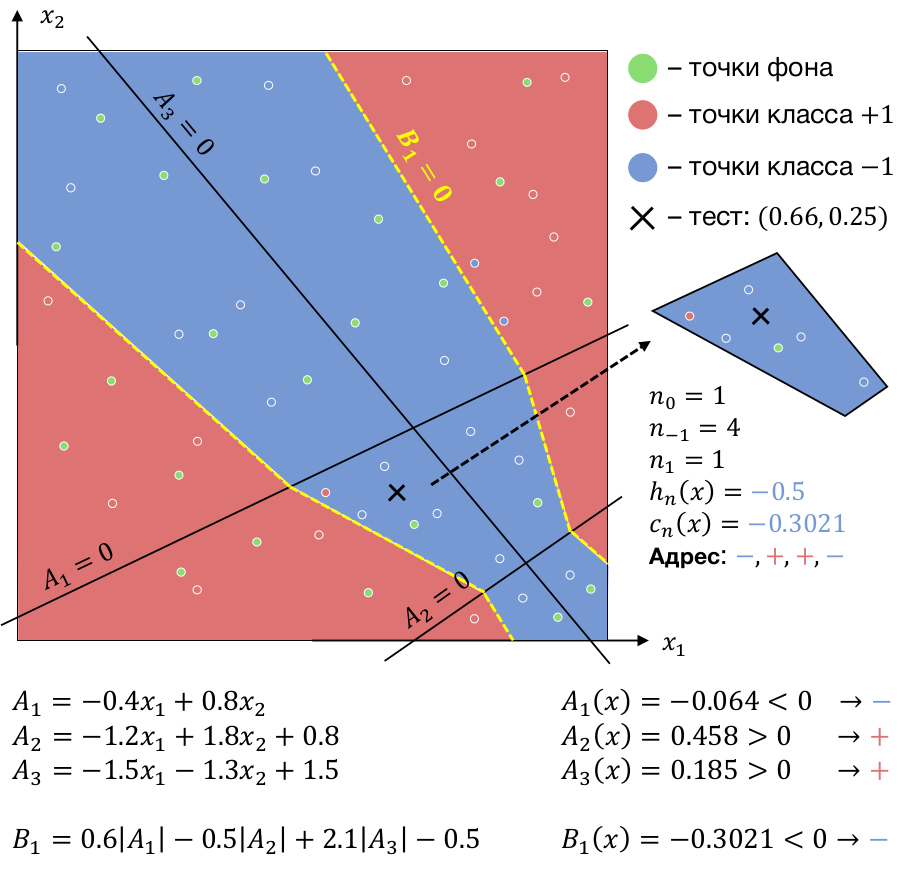
\includegraphics[width=\linewidth]{Dissertation/images/ch1/exbtree/exbtree.png}
    }
    \caption{Пример eXBTree на основе персептрона с \(d = 2\), \(L = 1\), \(k = 3\)}
    \label{fig:exbtree_example}
\end{figure}

Наличие такой структуры позволяет не только интерпретировать классификацию конкретного наблюдения (путь через дерево), но и формировать иерархию разбиений пространства, объединяя соседние ветви дерева на разных уровнях. Это открывает возможности для оценки доверия и анализа прецедентов -- как в пределах отдельной ячейки, так и на объединённых областях пространства.

%%%%%%%%%%%%%%%%%%%%%%%%%%%%%%%%%%%%%%%%%%%%%%%%%%%%%%%%%%%%%%%%%%%%%%%%%%%%%%%%%%%%%%%%%%%%%%%%%%%%%%%%%%%%%%%
\subsection{Комбинаторная сложность и практическая реализация eXBTree}

\begin{theorem}[О сложности построения дерева по многослойному персепртону]
    Пусть многослойный персептрон состоит из \(L\) скрытых слоёв по \(k\) нейронов в каждом (\(k > d\), где \(d\) -- размерность входного пространства). Тогда временная сложность построения двоичного дерева решений по персептрону составляет \(\mathcal{O}(k^{dL})\).
\end{theorem}
\fixme{ДОКАЗАТЕЛЬСТВО}

Тем не менее, в рамках задач классификации или аппроксимации нас интересуют не все возможные ячейки, а лишь те, в которые попали обучающие (или тестовые) наблюдения. Таким образом, нет необходимости в полном построении дерева. Достаточно определить множество фактически реализованных путей, то есть таких комбинаций знаков при раскрытии модулей, которые соответствуют реально встречающимся входным точкам.

Это приводит к следующему практическому алгоритму: каждое наблюдение при прямом проходе через сеть порождает набор знаков уравнений нейронов (до применения активационной функции), который можно трактовать как адрес ячейки. Хранить необходимо лишь такие уникальные адреса, тем самым получая компактное и эффективное представление разбиения пространства, ограниченное данными.

\begin{theorem}[О временной сложности получения решения по построенному дереву]
    Временная сложность получения ответа по построенному дереву решения совпадает со сложностью применения многослойного персептрона и составляет \(\mathcal{O}(kd + Lk^2)\).
\end{theorem}
\fixme{ДОКАЗАТЕЛЬСТВО}

%%%%%%%%%%%%%%%%%%%%%%%%%%%%%%%%%%%%%%%%%%%%%%%%%%%%%%%%%%%%%%%%%%%%%%%%%%%%%%%%%%%%%%%%%%%%%%%%%%%%%%%%%%%%%%%
\subsection{Геометрический анализ построенного дерева}

Рассмотрим свойства дерева, построенного на основе модифицированного обучающего множества с фоновыми наблюдениями, описанного ранее. В каждом внутреннем узле такого дерева содержится линейное неравенство, возникающее из перехода через гиперплоскость активации некоторого нейрона персептрона \(c_n^*(X)\). Каждая вершина дерева соответствует определённой комбинации знаков выражений вида~\(a_i^\top x + a_0\) и, следовательно, описывает подмножество признакового пространства -- выпуклый многогранник, ограниченный системой линейных неравенств.

В каждом листе дерева подсчитывается число объектов обучающего множества, попавших в соответствующую ячейку, с разбиением по классам: \(n_{-1}\), \(n_0\) и \(n_{+1}\). Таким образом, каждый лист фактически содержит гистограмму классов, обсуждавшуюся в разделе~\cref{subsec:ch1/histogram_approximation}. Эти гистограммы позволяют оценивать апостериорные вероятности классов в пределах каждой ячейки и выявлять области с высокой или низкой степенью уверенности модели.

Полученное дерево может быть также рассмотрено как дерево решений с линейными функциями разделения в узлах~\cite{devyatkinpostroenie}, в отличие от традиционных деревьев, в которых узлы соответствуют пороговым условиям вида \(x_j < c\). Такое представление делает поведение многослойного персептрона интерпретируемым: каждый путь от корня до листа соответствует системе линейных неравенств, описывающих область пространства, где модель принимает определённое решение линейным образом.

Важно подчеркнуть, что данная структура обеспечивает интерпретируемость модели в геометрических терминах, что традиционно считается слабой стороной нейронных сетей~\cite{salih2024linear}. В частности, можно явно указать, при каких линейных соотношениях между признаками модель принимает то или иное решение, и каков уровень уверенности классификатора в пределах каждой ячейки. Это позволяет использовать построенное дерево не только как аппроксиматор функции принятия решений, но и как инструмент визуального и количественного анализа поведения модели в различных областях признакового пространства.

%%%%%%%%%%%%%%%%%%%%%%%%%%%%%%%%%%%%%%%%%%%%%%%%%%%%%%%%%%%%%%%%%%%%%%%%%%%%%%%%%%%%%%%%%%%%%%%%%%%%%%%%%%%%%%%
\subsection{Анализ прецедентов и локальной уверенности}

Для повышения интерпретируемости построенного дерева и повышения доверия пользователя к решению важным является анализ конкретных прецедентов -- обучающих объектов, попавших в ту же ячейку дерева, что и тестируемое наблюдение. Вместо представления лишь числового выхода модели (например, вероятности класса 0.98), полезно показать близкие по признаковому пространству точки из обучающей выборки, что даёт наглядное представление о локальном окружении и структуре данных. Таким образом, построенное дерево служит своеобразной псевдо-метрикой, определяющей локальную близость объектов на основе разбиения пространства признаков.

Каждый лист дерева соответствует области признакового пространства, ограниченной системой линейных неравенств. В пределах этой области подсчитывается статистика по объектам различных классов. Однако в реальных задачах, особенно в медицинских и других высокорисковых прикладных областях, объёмы доступных данных могут быть недостаточными для надёжной статистической оценки на уровне отдельных ячеек.

В таких случаях целесообразно рассматривать информацию о соседних ячейках того же уровня дерева. Соседями называются ячейки, отличающиеся значением только одного из предикатов на пути от корня. Если в рассматриваемой ячейке содержится недостаточное количество наблюдений (например, менее заданного порога \(n_\text{min}\)), то можно агрегировать информацию с её соседями для получения более устойчивой оценки локального распределения классов.

Альтернативным подходом является подъём на уровень выше по дереву, то есть укрупнение ячейки за счёт устранения одного из условий, ограничивающих пространство. Это приводит к рассмотрению более широкой области признакового пространства, в которой ожидается большее количество обучающих объектов. Полученная таким образом укрупнённая ячейка также может быть проанализирована с точки зрения гистограммы классов, как описано выше, обеспечивая оценку апостериорной вероятности при недостаточной локальной уверенности.

Подобная стратегия, основанная на анализе прецедентов, позволяет реализовать согласованную схему оценки доверия к решению модели: в случае низкой уверенности по статистике на текущем уровне происходит адаптивное укрупнение области анализа. Это даёт практический механизм для отказа от принятия решения в условиях недостаточной информации и одновременно повышает надёжность выводов, что особенно важно в высокорисковых прикладных задачах.
